% Slide: Tổng quan máy chủ
\begin{frame}{Máy chủ: Quản lý và Xử lý Dữ liệu Trung tâm}
    \begin{block}{Tổng quan}
        \begin{itemize}
            \item Máy chủ Python: \textbf{"Bộ não"} trung tâm, kết hợp dữ liệu từ:
            \begin{enumerate}
                \item \textbf{ESP32}: Trạng thái té ngã, GPS qua MQTT.
                \item \textbf{Camera IP}: Phát hiện người, theo dõi, ước lượng tư thế bằng AI.
            \end{enumerate}
            \item Hợp nhất dữ liệu để quyết định té ngã đáng tin cậy, kích hoạt cảnh báo, ghi sự kiện.
        \end{itemize}
    \end{block}
    \label{sec:server_overview}
\end{frame}

% Slide: Kiến trúc hệ thống
\begin{frame}{Máy chủ: Kiến trúc hệ thống}
    \begin{block}{Mô hình phân tầng}
        \begin{itemize}
            \item \textbf{Lớp thu nhận}: \texttt{comm/} (MQTT, Telegram, AMI), \texttt{detection/} (video camera).
            \item \textbf{Lớp xử lý}: \texttt{fall/}, \texttt{processing/} kết hợp dữ liệu.
            \item \textbf{Lớp đầu ra}: \texttt{database/} ghi sự kiện, \texttt{comm/} gửi cảnh báo.
        \end{itemize}
    \end{block}
    \label{subsubsec:system_overview}
\end{frame}

% Slide: Cấu trúc các mô-đun
\begin{frame}{Máy chủ: Cấu trúc các mô-đun}
    \begin{columns}[t]
        \begin{column}{0.48\textwidth}
            \begin{block}{Input \& Processing}
                \begin{itemize}
                    \item \texttt{comm/}: MQTT, Telegram, AMI.
                    \item \texttt{detection/}: Phát hiện người, theo dõi.
                    \item \texttt{fall/}: Phát hiện té ngã.
                    \item \texttt{processing/}: Kết hợp dữ liệu.
                \end{itemize}
            \end{block}
        \end{column}
        \begin{column}{0.48\textwidth}
            \begin{block}{Support \& Output}
                \begin{itemize}
                    \item \texttt{database/}: Lưu \texttt{fall\_events.db}.
                    \item \texttt{config/}, \texttt{models/}: Cấu hình, YOLOv8n.
                    \item \texttt{utils/}, \texttt{tests/}: Công cụ, kiểm tra.
                    \item \texttt{main.py}: Vòng lặp chính.
                \end{itemize}
            \end{block}
        \end{column}
    \end{columns}
    \label{tab:server_modules}
\end{frame}

% Slide: Luồng xử lý máy chủ
\begin{frame}[fragile]{Máy chủ: Luồng xử lý}
    \begin{figure}
        \centering
        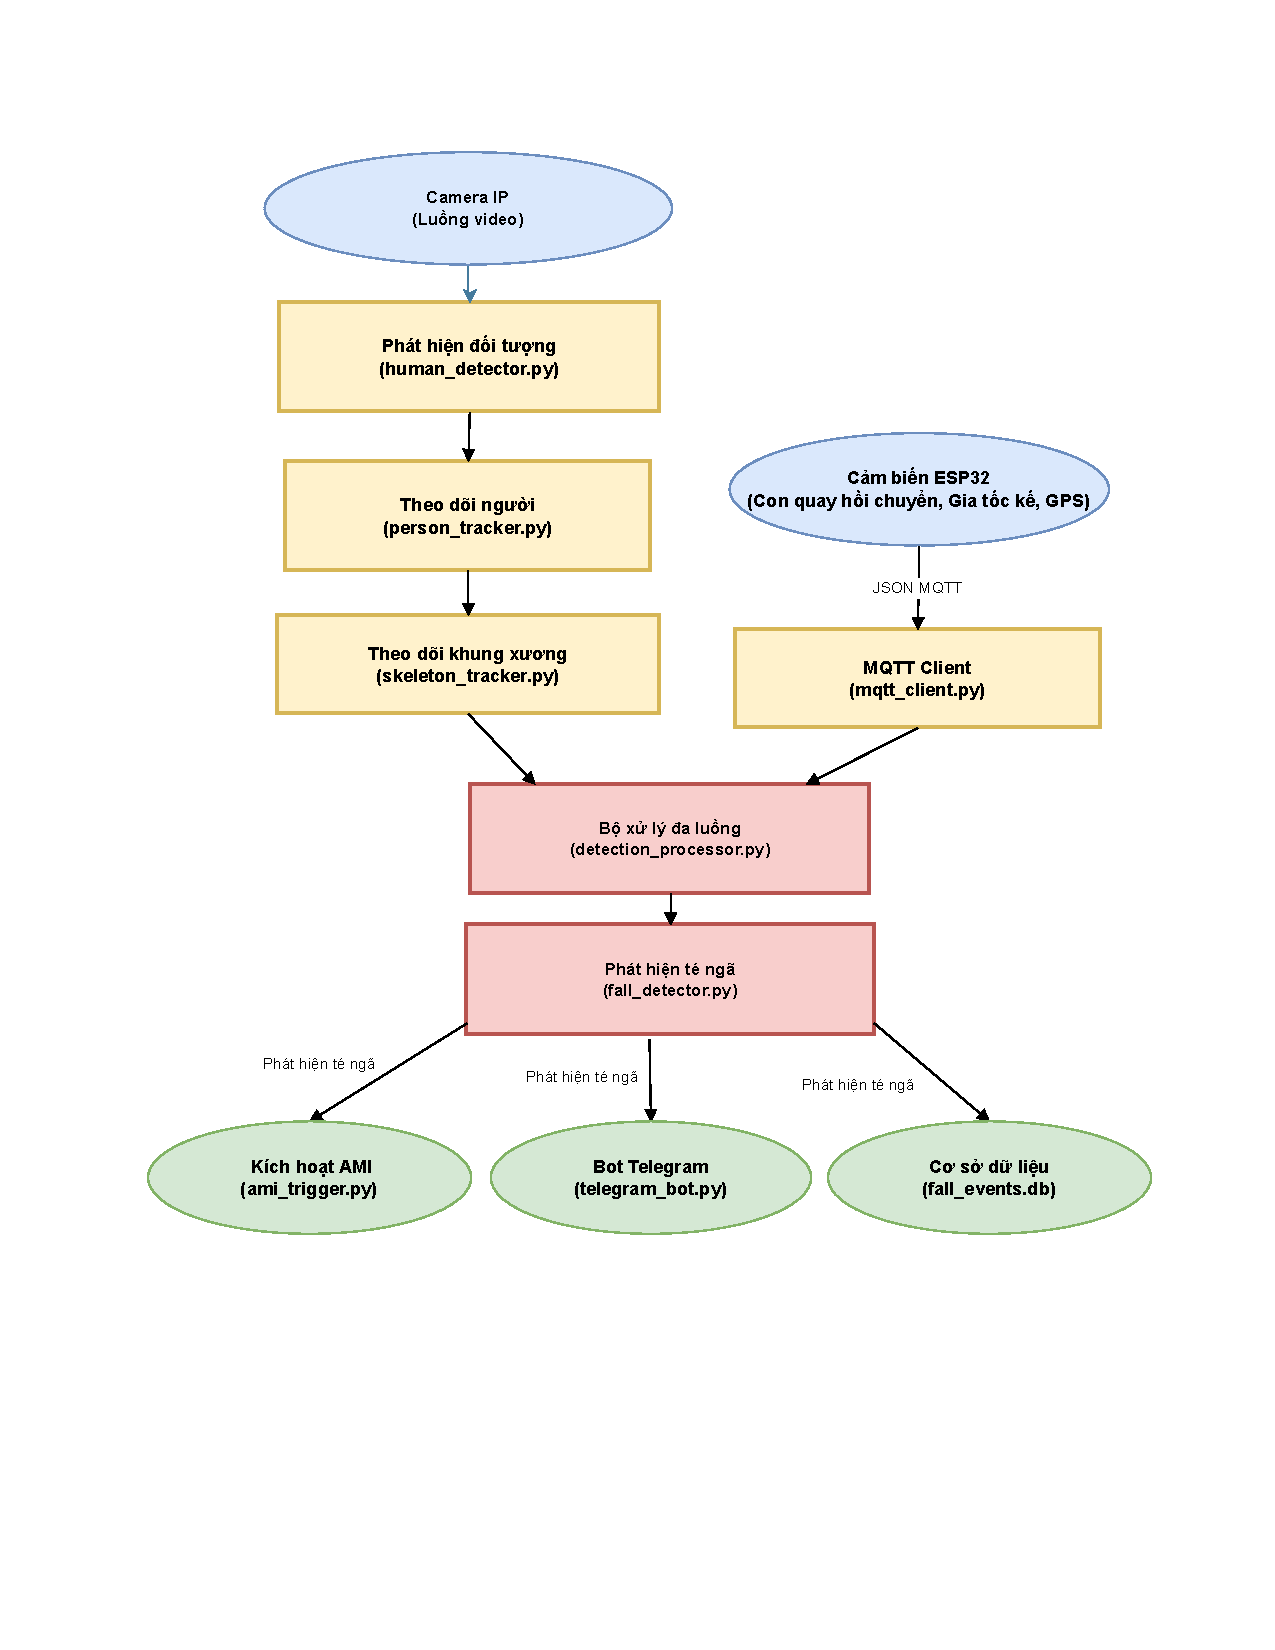
\includegraphics[width=0.85\textwidth,height=0.7\textheight,keepaspectratio]{images/server_flow.pdf}
        \caption{Luồng dữ liệu: Kết hợp ESP32 và Camera IP qua \textbf{DetectionProcessor}.}
        \label{fig:server_flow}
    \end{figure}
\end{frame}

% Slide: Kết hợp dữ liệu đa phương thức
\begin{frame}{Máy chủ: Kết hợp dữ liệu đa phương thức}
    \begin{block}{Quy trình}
        \begin{itemize}
            \item Thu nhận: MQTT JSON (ESP32), AI (camera).
            \item Đồng bộ: Dựa trên timestamp.
            \item Kết hợp: Logic AND/OR với trọng số độ tin cậy.
            \item Kích hoạt: Cảnh báo và ghi sự kiện.
        \end{itemize}
    \end{block}
    \label{subsubsec:multi_input_fusion}
\end{frame}

% Slide: Thuật toán phát hiện té ngã
\begin{frame}{Máy chủ: Thuật toán phát hiện té ngã}
    \begin{block}{Quy trình}
        \begin{itemize}
            \item \textbf{Kiểm tra}: Landmarks hợp lệ.
            \item \textbf{Tính toán}: Góc thân người (vai-hông), vận tốc.
            \item \textbf{Trạng thái}: 
                \begin{itemize}
                    \item \textit{Falling}: Góc + vận tốc vượt ngưỡng.
                    \item \textit{Lying}: Góc ngang kéo dài.
                \end{itemize}
            \item \textbf{Quyết định}: Bộ đếm vượt ngưỡng → té ngã, reset.
        \end{itemize}
    \end{block}
\end{frame}

% Slide: Lưu đồ thuật toán
\begin{frame}[fragile]{Máy chủ: Lưu đồ thuật toán}
    \begin{figure}
        \centering
        \includegraphics[width=0.85\textwidth,height=0.7\textheight,keepaspectratio]{images/python_fall_diagram.pdf}
        \caption{Lưu đồ giải thuật phát hiện té ngã trong Python.}
        \label{fig:python_fall_diagram}
    \end{figure}
\end{frame}

% Slide: Lưu trữ và cảnh báo
\begin{frame}{Máy chủ: Lưu trữ và cảnh báo}
    \begin{block}{Cơ chế}
        \begin{itemize}
            \item \textbf{Lưu trữ}: SQLite \texttt{fall\_events.db} (timestamp, confidence, sensor/pose data).
            \item \textbf{Cảnh báo}: Telegram/AMI khi phát hiện té ngã.
            \item \textbf{Vòng lặp}: Thu thập → AI xử lý → Kết hợp → Alert nếu cần.
        \end{itemize}
    \end{block}
    \label{subsubsec:data_storage_alerts}
\end{frame}

% Slide: Cấu trúc thư mục dự án
\begin{frame}[fragile]{Máy chủ: Cấu trúc thư mục dự án}
    \renewcommand{\baselinestretch}{0.8}
    \begin{minted}[fontsize=\scriptsize, breaklines, bgcolor=lightgray]{text}
intergrate_fall/
├── comm/ (MQTT, Telegram, AMI)
├── config/ (cấu hình)
├── database/ (fall_events.db)
├── detection/ (human, tracker)
├── fall/ (fall_detector.py)
├── processing/ (detection_processor.py)
├── utils/ (draw_utils.py)
├── models/ (yolov8n.pt)
├── tests/ (test_fall.py)
├── main.py
    \end{minted}
    \renewcommand{\baselinestretch}{1.0}
    \label{subsubsec:project_structure}
\end{frame}
